\RequirePackage{luatex85}
\documentclass[border=1pt]{standalone}
\usepackage{tikz}
\usepackage{siunitx}
\usetikzlibrary{shapes.geometric, arrows}

%%%%%%%%%%%%%%%%%%%%%%%%%%%%%%%%%%%%%%%%%%%%%%%%%%%%%%%%%%%%%%%%%%%%%%%%%%%%%%%%
%%%%%%%%%%%%%%%%%%%%                 colours                %%%%%%%%%%%%%%%%%%%% 
%%%%%%%%%%%%%%%%%%%%%%%%%%%%%%%%%%%%%%%%%%%%%%%%%%%%%%%%%%%%%%%%%%%%%%%%%%%%%%%%

\definecolor{tugreen}{RGB}{128, 186, 38}
\definecolor{tucitron}{RGB}{249, 219, 0}



%%%%%%%%%%%%%%%%%%%%%%%%%%%%%%%%%%%%%%%%%%%%%%%%%%%%%%%%%%%%%%%%%%%%%%%%%%%%%%%%
%%%%%%%%%%%%%%%%%%%%                 Boxes                  %%%%%%%%%%%%%%%%%%%% 
%%%%%%%%%%%%%%%%%%%%%%%%%%%%%%%%%%%%%%%%%%%%%%%%%%%%%%%%%%%%%%%%%%%%%%%%%%%%%%%%
\tikzstyle{normalBox} = [shape=rectangle, draw=black, text=black, thick, 	
	align=center, fill=white]

\tikzstyle{roundBox} = [shape=circle, draw=black, text=black, thick, 	
	align=center, fill=white]

\tikzstyle{alternBox} = [shape=rectangle, text=white, thick, align=center, 
	fill=black, rounded corners]


%%%%%%%%%%%%%%%%%%%%%%%%%%%%%%%%%%%%%%%%%%%%%%%%%%%%%%%%%%%%%%%%%%%%%%%%%%%%%%%%
%%%%%%%%%%%%%%%%%%%%                 Arrows                 %%%%%%%%%%%%%%%%%%%% 
%%%%%%%%%%%%%%%%%%%%%%%%%%%%%%%%%%%%%%%%%%%%%%%%%%%%%%%%%%%%%%%%%%%%%%%%%%%%%%%%

\tikzstyle{normalArrow} = [thick,->,>=stealth, draw=black]

\usepackage[utf8]{inputenc}
\usepackage[T1]{fontenc}
\usepackage[sfdefault]{FiraSans}


\tikzstyle{NormalBox} = [normalBox, text width =2.4cm, minimum height=0.9cm]
\tikzstyle{AlternBox} = [alternBox, text width =3.4cm, minimum height=0.9cm]

\begin{document}
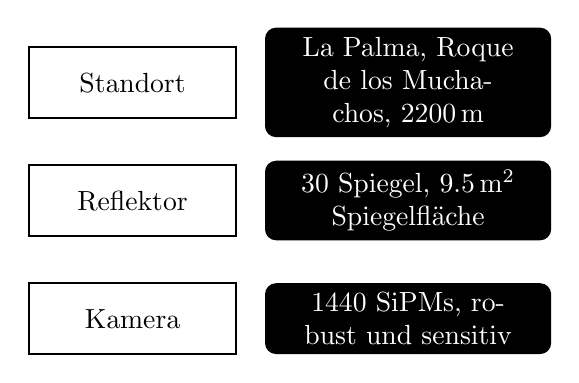
\begin{tikzpicture}[node distance=1.5cm]
  \node (LOC) [NormalBox] {Standort};
  \node (REF) [NormalBox, below of=LOC] {Reflektor};
  \node (KAM) [NormalBox, below of=REF] {Kamera};

  \node (Loc) [AlternBox, right of=LOC, xshift=2cm] {La Palma, Roque de los Muchachos, \SI{2200}{\meter}};
  \node (Ref) [AlternBox, right of=REF, xshift=2cm] {\num{30} Spiegel, \SI{9,5}{\meter\squared} Spiegelfläche};
  \node (Kam) [AlternBox, right of=KAM, xshift=2cm] {\num{1440} SiPMs, robust und sensitiv};

\end{tikzpicture}
\end{document}
